\documentclass[a4paper,headsepline,11pt]{scrartcl}


\usepackage{scrlayer-scrpage}
\usepackage{graphicx}
\graphicspath{{../fig/}}
\usepackage{caption}
\usepackage{subcaption}
%\usepackage{placeins}		%allows FloatBarrier command
\usepackage{amsmath, amssymb, amsthm}
\usepackage{bm}				%allows bm command for boldfaced vectors in math mode
\usepackage[utf8]{inputenc}
\usepackage[T1]{fontenc}
\usepackage{import}
\usepackage{float}
\usepackage{multirow}
%\usepackage{epstopdf}		%converts every .eps-file to a .pdf-file, which can then be included
\usepackage{booktabs}		%table_package
\usepackage{url}
%\usepackage[numbers,square,sort&compress]{natbib}

\usepackage{geometry}
\geometry{margin=2cm}

\usepackage{physics}
\usepackage[version=4]{mhchem}

\newcommand{\s}[1]{\mathrm{#1}}
\newcommand{\bs}[1]{\boldsymbol{#1}}
\newcommand*\diff{\mathop{}\!\mathrm{d}}
%colon equal sign
\mathchardef\ordinarycolon\mathcode`\:
\mathcode`\:=\string"8000
\begingroup \catcode`\:=\active
  \gdef:{\mathrel{\mathop\ordinarycolon}}
\endgroup


\usepackage{scrlayer-scrpage}
\automark*{section}
\clearpairofpagestyles
\ihead{\headmark}
\ohead{\pagemark}

%%%%%%%%%%%%%%%%%%%%%%%%%%%%%%%%%%%%%%%%%%%%%%%%%%%%%%%%%%%%%%%

%colorful linking within a PDF-Viewer
\usepackage{hyperref}
\hypersetup{
    colorlinks=true,
    linkcolor=blue,
    filecolor=magenta,
    urlcolor=cyan,
}

\title{Working Title: Reverse Design of Meta-surface Stacks via Neural Network}
\author{Tim Turan}
\date{\today}



%%%%%%%%%%%%%%%%%%%%%%%%%%%%%%%%%%%%%%%%%%%%%%%%%%%%%%%%%%%%%%%%%%%%%%%%%%%%

\begin{document}

\maketitle

\clearpage

\section{Abstract}
I hope this all works jada jada jada
Lorem ipsum dolor sit amet, consectetur adipisicing elit, sed do eiusmod tempor incididunt ut labore et dolore magna aliqua. Ut enim ad minim veniam, quis nostrud exercitation ullamco laboris nisi ut aliquip ex ea commodo consequat. Duis aute irure dolor in reprehenderit in voluptate velit esse cillum dolore eu fugiat nulla pariatur. Excepteur sint occaecat cupidatat non proident, sunt in culpa qui officia deserunt mollit anim id est laborum.

\clearpage

\tableofcontents
\clearpage

\section{Physical Background}
\subsection{$S$-Matrix Calculus} \label{sec:s_mats}
\subimport{./}{s_mats.tex}
\clearpage

\subsection{Neural Networks} \label{sec:NN_bg}
\subimport{./}{neural_networks_background.tex}

\clearpage

\section{The Algorithm}
\begin{figure}[H]
    \centering
    \includegraphics[width=.9\linewidth]{al_algo}
    \captionsetup{singlelinecheck=off}
    \caption[]{A Flowchart of the Algorithm
    \begin{description}
        \item[\protect{\parbox[t]{0.2\linewidth}{NN}}]
        \parbox[t]{0.8\linewidth}{convolutional neural ntwork trained to map spectra to stack and layer \\ parameters}
        \item[\protect{\parbox[t]{0.2\linewidth}{DB}}]
        \parbox[t]{0.8\linewidth}{database of FMM simulated single layers}
        \item[\protect{\parbox[t]{0.2\linewidth}{SASA}}]
        \parbox[t]{0.8\linewidth}{algorithm calculating $\hat{S}_\s{stack} = \hat{S}_\s{stack}(\hat{S}_1, \, \hat{S}_2, \, ...)$}
        \item[\protect{\parbox[t]{0.2\linewidth}{Opt}}]
        \parbox[t]{0.8\linewidth}{optimizer changing parameters to minimize the difference between the current and target spectrum}
        \item[\protect{\parbox[t]{0.2\linewidth}{$\bm{\hat{S}_1}, \, \bm{\hat{S}_2}$}}]
        \parbox[t]{0.8\linewidth}{S-matrices of the top and bottom layer}
        \item[\protect{\parbox[t]{0.2\linewidth}{layer\\params}}]
        \parbox[t]{0.8\linewidth}{these include the geometry of the periodic meta surface cell and the kind of material used}
        \item[\protect{\parbox[t]{0.2\linewidth}{stack\\params}}]
        \parbox[t]{0.8\linewidth}{the rotation angle of the layers to one another and the distance between}
        \item[\protect{\parbox[t]{0.2\linewidth}{new\\params}}]
        \parbox[t]{0.8\linewidth}{the Opt. only changes the continuous parameters, the discrete ones , e.g. material, remain unchanged}
        \item[\protect{\parbox[t]{0.2\linewidth}{optimization\\loop}}]
        \parbox[t]{0.8\linewidth}{this loop is repeated until the target accuracy is reached}
    \end{description}}
    \label{fig:al:algo}
\end{figure}

\clearpage

\section{The Neural Network}
\clearpage

\section{The Optimizer}
\clearpage

\section{Results}
\clearpage


\section{Literaturverzeichnis}
\bibliographystyle{unsrt}
\bibliography{../bib/}{sources.bib}

\clearpage

\section{Anhang}
\clearpage

\end{document}
